\chapter{Experimentelle Methoden}

\section {Metallografische Präparation (VR)}

\subsection*{Trennen}

Die wärmebehandelten Proben werden in der Mitte mit einer Siliziumkarbid-Scheibe unter ständigem Kühlmittelfluss im Querschliff getrennt (Trennmaschine Jean Wirtz CUTO 20). Durchgehende Kühlung  verhindert eine zusätzliche, ungewollte Gefügeveränderung an der Schnittfläche während des Trennvorgangs.


\subsection*{Einbetten}

Die getrennten Proben werden in Warmeinbettpressen (Buehler Simplimet Mounting Press 1000 und 4000) für bessere Handhabung und Stützung der Randzonen eingebettet. Beim Warmeinbetten wird mit Hilfe von Druck und Temperatur die Probe in ein Kunststoffgranulat eingeschlossen. Vorteile des Warmeinbettens sind die hohe Härte und Spaltfreiheit des Einbettmaterials. Dabei wird Epomet als erste Schicht im Bereich der Probenoberfläche benutzt und für die oberflächenfernen Bereiche Bakelit, da Epomet eine bessere Spaltfüllung hat. Das Warmeinbetten erfolgte mit den gerätespezifischen Parametern aus Tab.~\ref{tab:Einbettpressen}. 
Die fertig eingebetteten Proben werden entgratet und auf der Seite der Probenoberfläche mit einer Fase versehen.  


\begin{table}[h]
	\centering
	\begin{tabular} {|c|c|c|}
		\hline
		&Bühler Simplimet 1000 & Bühler Simplimet 4000 \\
		\hline
		Temperatur [$^\circ$C]&180&180 \\
		\hline
		Druck [bar]&200&290 \\
		\hline
		Heizzeit [min]&2&4.5 \\
		\hline
		Kühlzeit [min]&5&3.5 \\
		\hline
	\end{tabular}
	
	\caption{Einbettparameter für Bühler Simplimet 1000 und 4000}
	\label{tab:Einbettpressen}
\end{table}

\subsection*{Schleifen/Polieren}

Die Trennfläche der Proben wird in Vorbereitung auf die Ätzung der Oberfläche geschliffen und poliert. Ziel ist eine Oberfläche, die frei von Riefen und Fremdpartikeln ist. Als Schleif-/~Poliergerät wurde ein ATM Saphir 550 benutzt.
Im ersten Schritt werden die Proben mit steigender Körnung im Gegenlauf geschliffen und dabei wassergekühlt (siehe Tab. \ref{tab:Schleifstufen}). Der Probenhalter und Schleifteller haben beide eine Umdrehungszahl von 150 min$^{-1}$, die während des gesamten Schleif- und Polierprozesses gleich bleibt.   

\begin{table}[h]
	\centering
	\begin{tabular}{|c|c|c|c|c|c|c|c|c|}
		
		\hline 
		Körnung (FEPA P) & 180 & 240 & 320 & 400 & 600 & 800 & 1200 & 2500 \\ 
		\hline 
		Zeit [min] & 0:30 & 1:00 & 1:30 & 2:00 & 2:30 & 3:00 & 3:30 & 4:00 \\ 
		\hline 
		Anpressdruck [N] & 10&10&10&10&10&10&6&6\\
		\hline
	\end{tabular} 
	\caption{Schleifstufen}
	\label{tab:Schleifstufen}
\end{table}

Zwischen jeder Körnung werden die Proben drei Minuten in einer Seifenlauge ultraschallgereinigt, um größere Schneidkörner und Abrieb nicht zu verschleppen, und die Dauer des Schleifens um 30s verlängert. 

Zum Polieren wird eine Wabenscheibe mit destilliertem Wasser und einer Poliersuspension bestehend aus Oxid-Polier-Suspension (0.05$\mu$m) und Wasserstoffperoxid im Verhältnis 5:1 benetzt. Jede Minute wird Poliersuspension nachgegeben, um eine kontinuierliche Politur zu gewährleisten.

\begin{table}[h]
	\centering
	
	\begin{tabular}{|c|c|c|c|}
		\hline 
		Schritt & Druck [N] & Zeit [min] & Richtung \\ 
		\hline 
		1 & 7 & 5 & Gegenlauf \\ 
		\hline 
		2 & 5 & 2 & Gleichlauf \\ 
		\hline 
	\end{tabular} 
	\caption{Polierstufen}
	\label{tab:Polierstufen}
\end{table}

Die Proben werden nach jedem Schritt (siehe Tab. \ref{tab:Polierstufen}) vier Minuten in einem Ethanolbad ultraschallgereinigt. Nach beiden Polierschritten wird die Wabenscheibe mit Spülmittel gesäubert und die Schritte 1 und 2 wiederholt. Es wird solange poliert bis die Probenoberfläche frei von Riefen und Fremdpartikeln ist. Im letzten Schritt wird die Probenoberfläche nach der Ultrasschallreinigung mit Spülmittel und anschließend mit Ethanol gereinigt und getrocknet. 



\subsection*{Ätzen}

Im letzten Schritt der Probenpräparation werden die Oberflächen der Trennfläche geätzt. Die polierte Oberfläche der Proben reflektiert Licht nahezu gleichmäßig, wodurch das Gefüge der Legierung nicht zu erkennen ist. Das Ätzen erzeugt einen Kontrast zwischen den verschiedenen Mikrostrukturen des Gefüges durch die unterschiedlichen Korrosionsraten der einzelnen Bestandteile \cite{Lutjering.2007}. Stärker korrodierte Gefügebestandteile sind dunkler bei lichtmikroskopischer Betrachtung.
Die Proben werden in einem Ätzmedium nach Kroll (siehe Tab. \ref{tab:Ätz_Kroll}) 7s, martensitische Proben 10s lang geätzt. 

\begin{table}
	\centering
	\begin{tabular}{|c|c|}
		
		\hline 
		Destilliertes Wasser
		& 100ml
		\\ 
		\hline 
		Salpetersäure (HNO$_{3}$)	& 6ml
		\\ 
		\hline 
		Flusssäure (HF) & 3ml
		\\ 
		\hline 
	\end{tabular} 
	\caption{Ätzlösung nach Kroll}
	\label{tab:Ätz_Kroll}
\end{table}

\section{Untersuchung der Mikrostruktur (TJ)}

\subsection*{Lichtmikroskopie}

Nach der Probenpräparation werden die Proben unter dem Lichtmikroskop untersucht. Für die Untersuchung wurde das Zeiss AX10 Lichtmikroskop verwendet. Es werden Bilder mit 200-facher bis 1000-facher Vergrößerung aufgenommen, welche mit ihrem Datennamen und Auflösung beschriftet werden. Anschließend werden verschiedene Stellen untersucht, um die Mikrostrukturen der Proben besser erfassen zu können.

Die einzelnen Phasenanteile können mit Hilfe der verschiedenen Graustufen differenziert und analytisch ausgewertet werden. Dazu können Filter eingesetzt werden, um bestimmte Mikrostrukturen besser hervorzuheben. Es werden \textit{Differential Interference Contrast in circularly polarized lights} (C-DIC) benutzt. Sie sorgen für eine sehr hohe Kontrastdifferenz. Bei mehrphasigen Proben werden sie häufig verwendet, da durch eine Polarisation des Lichtes die Gefüge, insbesondere die Korngrößen- und Phasenanteilbestimmung, optisch besser auswertbar sind.

\subsection*{Rasterelektronenmikroskopie (REM)}

Das Rasterelektronenmikroskop wird benutzt, um eine dreidimensionale Darstellung der Oberfläche zu erzeugen. Das REM Hitachi Tabletop Microscope TM3000 steht mit zwei Freiheitsgraden zur Verfügung (X-, Y-Richtung). Das Mikroskop ermöglicht höhere Auflösungen gegenüber dem Lichtmikroskop und bietet die Möglichkeit Oberflächen, Materialien sowie die chemische Zusammensetzung zu analysieren. 

Die Proben werden in einer Vakuumkammer untersucht. Im REM werden Elektronen zwischen einer Anode und einer Kathode durch eine angelegte Spannung beschleunigt. Mit Hilfe von magnetischen Linsen werden die ausgestrahlten Elektronen auf die Probenoberfläche fokussiert. 
Die Elektronen, die von der Probenoberfläche zurückkommen, werden detektiert und zu einem Bild verabeitet. 
Um dieses Bild zu erzeugen, werden ausgeschlagene sekundäre Elektronen (SE) detektiert. Diese SE Informationen werden aus der Oberfläche entnommen und in ein Abbild umgewandelt. 
Es lässt sich damit eine dreidimensionale Darstellung der Probenoberfläche erzeugen, je nach Topographie der untersuchten Fläche.

Unter anderen kann das REM mehrere Informationen über die Probe verarbeiten. Eine Veranschaulichung des Massenverhältnisses der Elemente wird mit dem Rückstreuelektronen-Detektor (\textit{Backscatter Electrons}, BSE) bestimmt. Unterschiedliche Phasen erzeugen aufgrund ihrer chemischen Zusammensetzung unterschiedlich starke Kontraste. Die Helligkeit der Bilder wird durch die Anzahl der Elektronen bestimmt.

Die chemische Zusammensetzung der Legierung kann mithilfe der Energiedispersiven Röntgenspektroskopie (EDX) erfasst wird. Aus den inneren Schalen der Atome werden Elektronen ausgestoßen, wodurch Energie freigesetzt wird. Diese Energie wird bei einer EDX-Analyse mit Hilfe eines Siliziumkristalls, der mit flüssigem Stickstoff gekühlt wird, gemessen. Das entstehende Spektrum zeigt dann die Zusammensetzung der Legierung. Es werden an unterschiedlichen Stellen der Probe Flächenanalysen erstellt, um möglichst genaue Daten zu erhalten.

\subsection*{\textit{Field emission} REM}
Für eine bessere Auflösung bei hoher Vergrößerung steht der Smart SEM LEO 1550 zur Verfügung. Die Probenaufnahme der Prozesskammer besitzt 5 Freiheitsgrade (X-, Y-, Z-Richtung, Neigung, Rotation) und mit dem Programm Gemini betrieben. Die Bilder sind entweder mit SE-Detektoren (SE2) erzeugt, oder mit dem Inlens Detektor (hohe Auflösung). Das FE REM hat einen ähnlichen Aufbau und funktioniert wie das zuvor erklärte REM.

Es werden Bilder an verschiedenen Stellen der Probe aufgenommen. Im Mittelbereich und am Rand werden diese mit 2000- bis 20000-facher Vergrößerung untersucht. Polierartefakte können bei der Analyse mit Gefügebestandteilen verwechselt werden. 

\subsection*{$\alpha_{p}$-Volumenanteil Analyse}

Die Bilder vom Lichtmikroskop werden mit Hilfe des Bildbearbeitungsprogramms GIMP analysiert. Zunächst werden die Phasen auf den Bildern durch gezielte Kontrasteinstellung voneinander abgehoben. Im Histogramm können dann die durch die unterschiedlichen Graustufen repräsentierten Gefügebestandteile abgelesen werden. Durch die Analyse von acht verschiedenen Stellen wird ein Mittelwert des $\alpha_{p}$-Volumenanteils mit einer Genauigkeit von 3\% ausgewertet.


\section{Mechanische Prüfverfahren (VR)}

\subsection*{Härteprüfung}

Die Härte der Proben wurde mit einer Vickers-Prüfung nach DIN Norm 50133 ermittelt. Dabei wird die Eindringhärte des Materials gegenüber eines Eindringkörpers in Form einer gleichseitigen Diamantpyramide gemessen. Die Diamantpyramide hat einen Öffnungswinkel von $136^\circ$ zwischen den Seitenflächen und wird mit 10 kg (98,1 N) statischem Druck 15 s lang in die Probe gedrückt. Über die gesamte Probenlänge verteilt werden fünf Eindrücke erzeugt. Ein Abstand von mindestens dreimal der Eindruckdiagonalen $d$ muss dabei vom Rand und zwischen den Eindrücken eingehalten werden.
Die Eindrücke positioniert der Bediener anhand einer lichtmikroskopoischen Aufnahme mit geringer Vergrößerung in der Software. Mit vergrößerten Aufnahmen der ausgewählten Positionen lässt sich der Fokus auf die Bildebene festlegen. Die Prüfmaschine fertigt die Eindrücke automatisch an und fotografiert diese. Die Software ermittelt die Längen der Diagonalen $d_1$ und $d_2$. Dabei kann eine manuelle Überprüfung des von der Software gewählten Messbereichs vorgenommen werden. Die Vickershärte wird durch

$$HV=\frac {2*0,102*F*\sin \left( \frac{136^\circ}{2}\right) } {d^2} \approx 0,1891 \frac{F}{d^2}$$

mit der Eindruckkraft $F$ in Newton und $d=\frac {d_1 + d_2}{2} $ berechnet. Es kann eine Genauigkeit bis auf 3\% erzielt werden.  Die Härte eines Werkstoffs lässt in den meisten Fällen einen direkten Rückschluss auf die Festigkeit zu. Damit kann ohne einen aufwendigeren Zugversuch eine Umwertung der Härte in die Zugfestigkeit anhand empirischer Werte vorgenommen werden. 

\subsection*{Zugversuch}
Zur Bestimmung wichtiger Werkstoffkennwerte wie der Bruchdehnung, Zugfestigkeit, Dehngrenze und des Elastizitätsmoduls werden Zugversuche durchgeführt. Der Zugversuch ist ein genormtes Standardverfahren (DIN EN ISO 6892-1 Teil B), das zu den quasistatischen, zerstörenden Prüfverfahren gehört. Nach DIN 50125-B5x25 in Größe und Form genormte Proben werden dabei mit einer Spannungsgeschwindigkeit von 10 MPas$^{-1}$ bis zum Bruch gedehnt. Gleichzeitig wird die Längenänderung $\Delta l$ und die Kraft $F$ an der Probe gemessen. Mit der Anfangslänge $l_0$ und dem Anfangsquerschnitt $S_0$ lassen sich Nennspannung $\sigma$ und die Dehnung $\epsilon$ berechnen.

$$\sigma=\frac{F}{S_0}$$

$$\epsilon=\frac{\Delta l} {l_0}$$

Die Nennspannung und Dehnung werden in einem Spannungs-Dehnungs-Diagramm (Abb. \ref{fig:spandehn}) gegeneinander aufgetragen. Das Elastizitätsmodul wird von der Messsoftware an der Stelle größter Steigung mit Hilfe einer Tangente berechnet. 

\begin{figure}
	\centering
	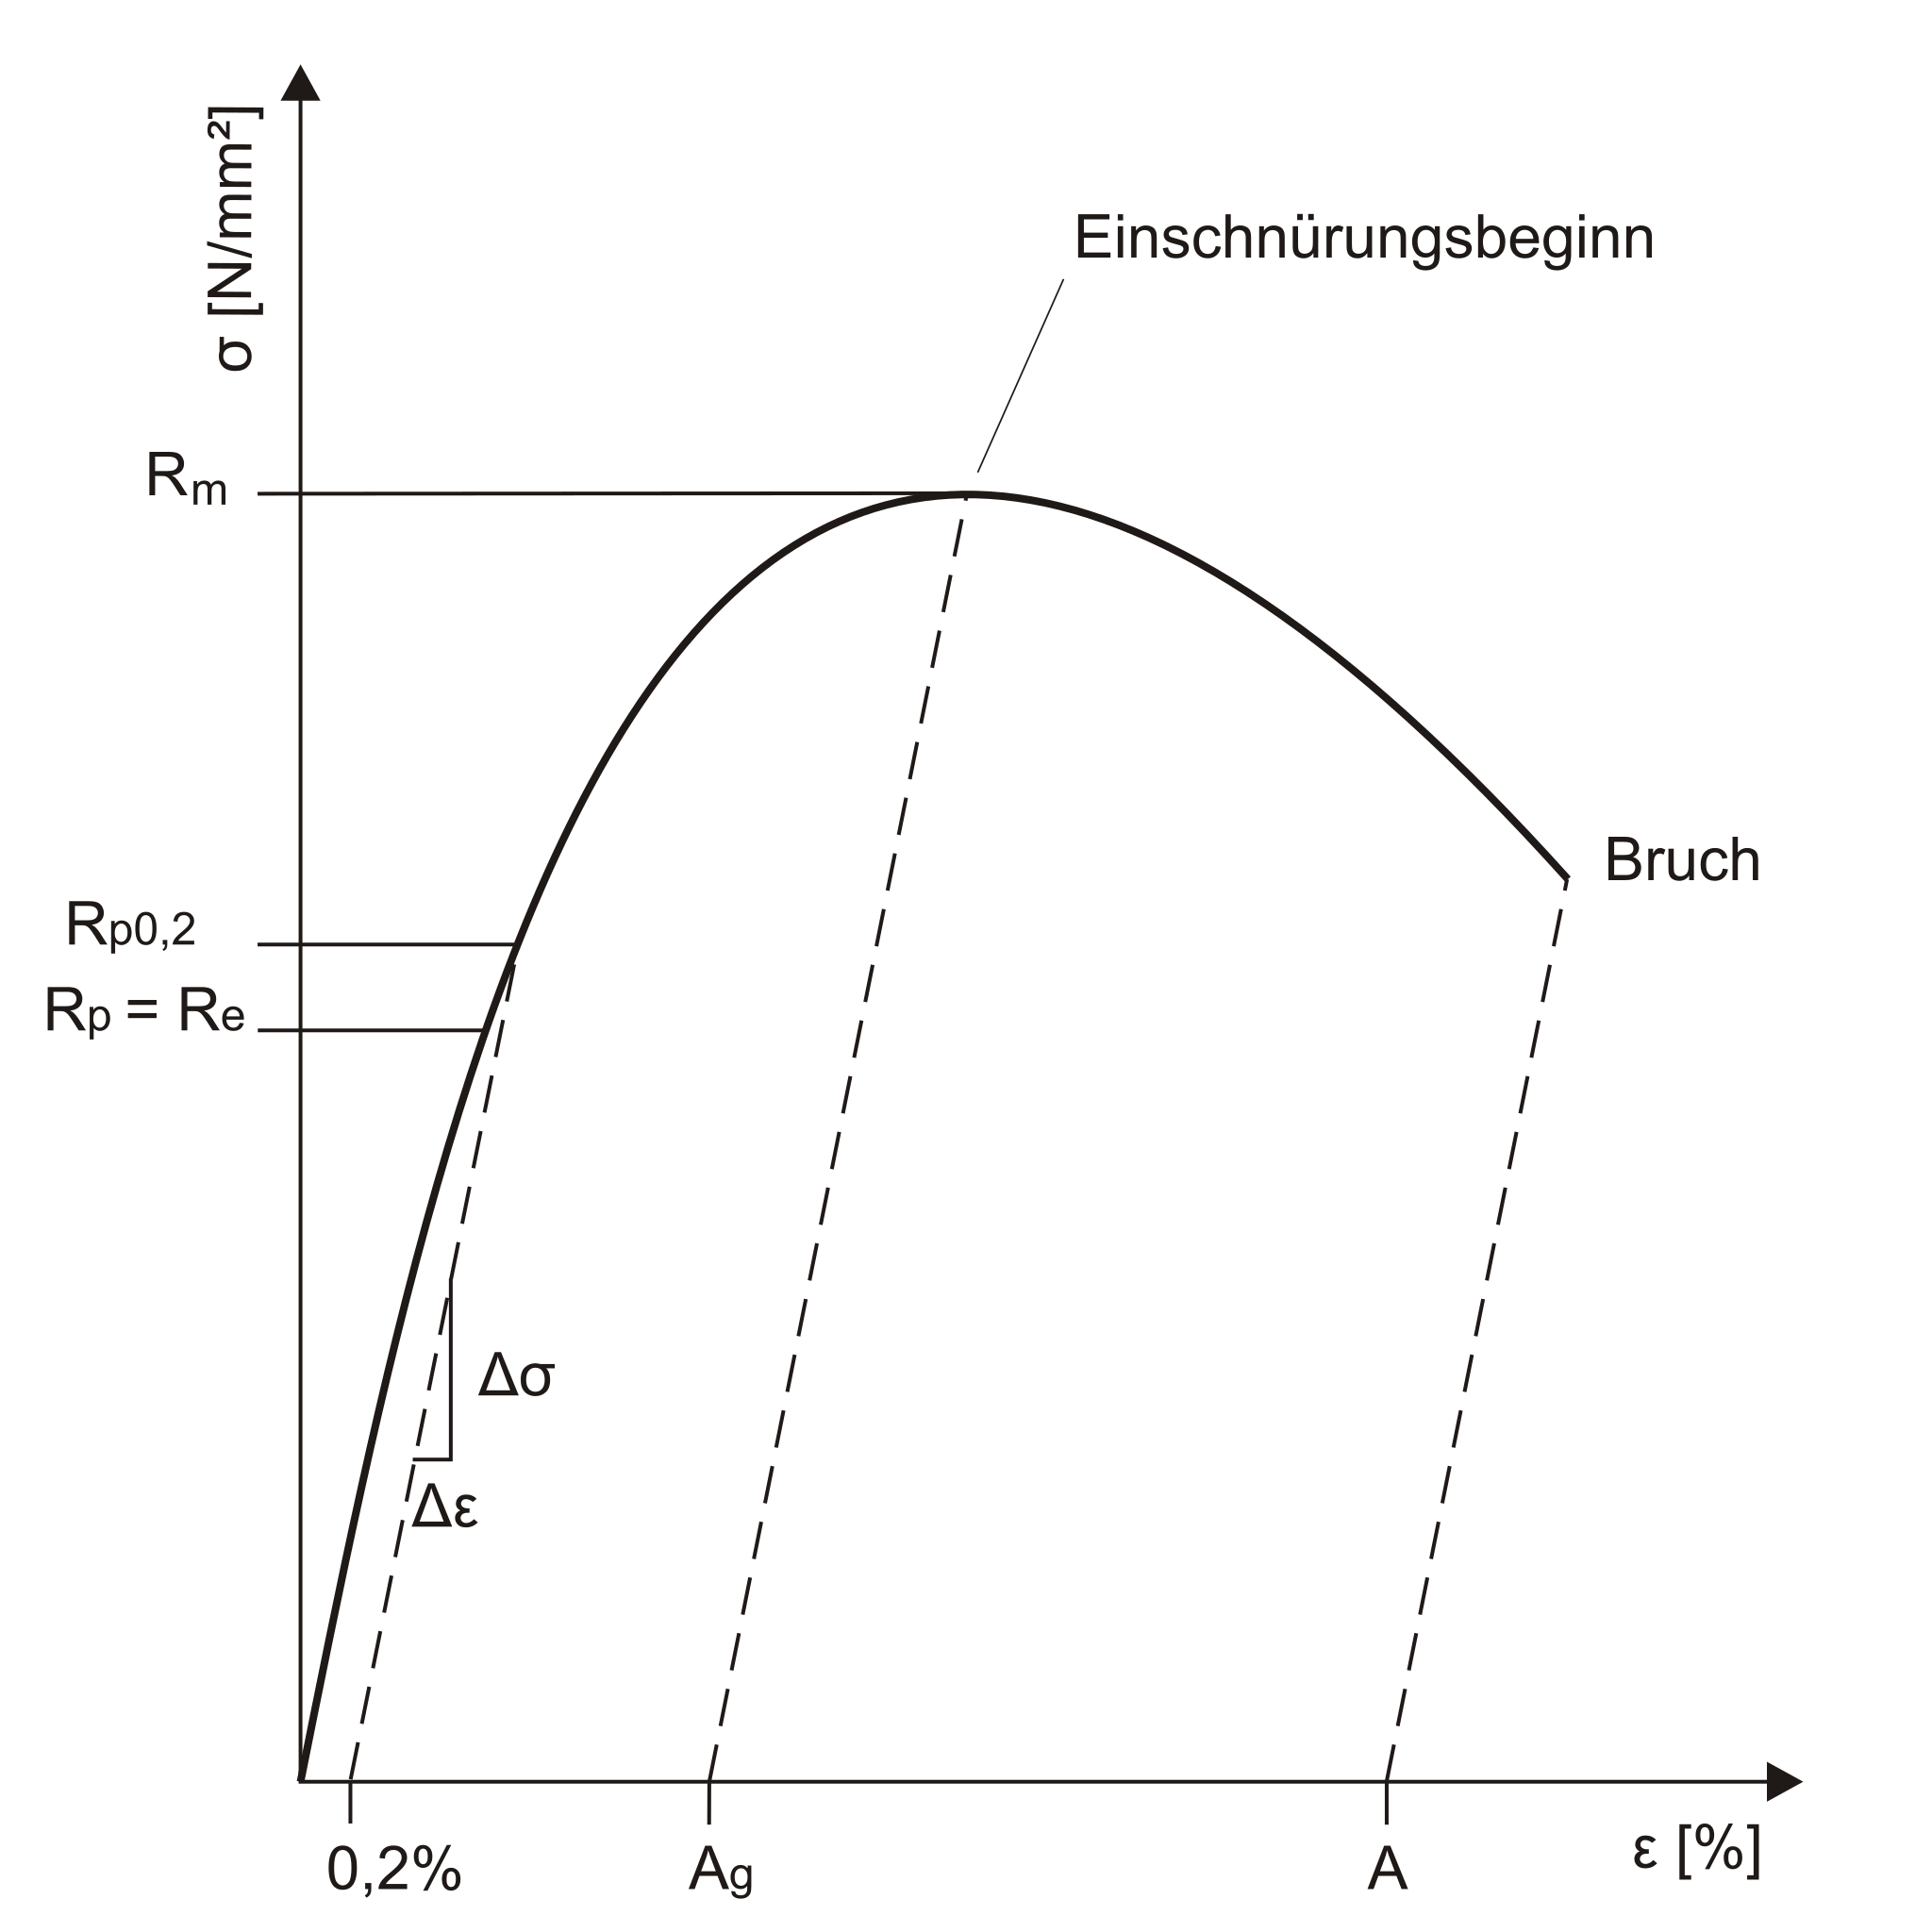
\includegraphics[width=0.6\linewidth]{./Bilder/Spgs-Dehnungs-Kurve_Dehngrenze}
	\caption{Spannungs-Dehnungs-Diagramm}
	\label{fig:spandehn}
\end{figure} 


